\documentclass[12pt]{article}

\usepackage{sbc-template}


\usepackage{graphicx}
\usepackage{pythontex} 
\usepackage[brazil]{babel}   
\usepackage[utf8]{inputenc}  
\usepackage{circuitikz}


\sloppy

\title{Análise do Circuito RC}

\author{Pedro Henrique Gomes\inst{1}, Sarah Pereira Cerqueira\inst{2} }


\address{Departamento de Tecnologia (DTEC) -- Universidade Estadual de Feira de Santana
  (UEFS)\\
  Caixa Postal 252 e 294 -- 44036-900 -- Feira de Santana -- BA -- Brazil
  \email{ peuh\_fsa@hotmail.com,
  sarahecomp@gmail.com}
}

\begin{document} 

\maketitle

\begin{resumo}
O presente documento faz uma análise do circuito RC em série  no domínio da frequência
\end{resumo}

 \section{Introdução}
 O circuito resistor-capacito (RC), é um dos filtros eletrônicos mais simples e básico da eletrônica. Ele consiste em um capacitor e um resistor ligados em série ou paralelo, alimentados por uma fonte de tensão. 
 
 Diferente de circuitos puramente resistivos, cuja aplicação das leis de Kirchhoff resulta numa equação algébrica, a aplicação das leis de Kirchhorff em um circuito RC produz uma equação diferencial de primeira ordem, que é mais difícil de resolver do que uma algébrica. 
 
 Ao alimentar o circuito RC com uma fonte senoidal de amplitude constante, variando a frequência obtemos a resposta em frequência do circuito, que pode ser considerada uma descrição completa do compotamento em regime estacionário senoidal de um circuito em função da frequência. 
 
 Neste trabalho será feita uma análise do ciruito RC em série, no domínio da frequência apresentando sua  função transferência.
 
 \section{ Metodologia}


\subsection{Diagrama do Circuito}

%DESENHO DO CIRCUITO
\begin{center}
\begin{circuitikz}[scale=1.6, transform shape][american voltages]
\draw 
(0,0){to[american voltage source, invert, l=$Vi$, color=red] (0,2) }
 to[R, l=$R$, i=$i$] (2,2)
 to[capacitor, v^>=$Vo$] (2,0) -- (0,0)
 ;\end{circuitikz}
 \end{center}

 %ANÁLISE DO CIRCUITO

 
 \subsection{Análise do Circuito}
A reatância e a Indutância num capacitor podem ser descritas por:

\begin{equation}
Xc = \frac{1}{w.C}\\
\end{equation}

\begin{equation}
Zc = Xc.j\\
\end{equation}

logo:

\begin{equation}
Zc = \frac{j}{w.C}\\
\end{equation}

Aplicando o divisor de Tensão:

\begin{equation}
Vo(w)=\frac{Zc.Vi}{Zc+Zr}
\end{equation}

Sabemos que a impedância Zr no resistor vale:

\begin{equation}
Zr= R
\end{equation}


Agora substituindo (3) em (4), 

\begin{equation}
Vo(w)=\frac{\frac{j.Vi}{w.C}}{\frac{j}{w.C} + R}
\end{equation}

Simplificando esse resultado, temos: 

\begin{equation}
Vo(w)=\frac{1.Vi}{1+jwRC}
\end{equation}

Portanto, a resposta em frequência desse circuito é expressa por:
\begin{equation}
\frac{Vo(w)}{Vi(w)}=\frac{1}{1+jwRC}
\end{equation}

Como solicitado, consideraremos R.C = 1, então temos:

\begin{equation}
\frac{Vo(w)}{Vi(w)}=\frac{1}{1+j.w}
\end{equation}

Por fim, fazendo \textit{s} = j.w o resultado final será:

\begin{equation}
\frac{Vo(s)}{Vi(s)}=\frac{1}{1+\textit{s}}
\end{equation}

\section{Conclusão}
A função transferência de um circuito é a razão, dependende da frequência, de uma saída para uma entrada, e é útil para encontrar a resposta em frequência de um circuito. No caso do circuito RC análisado, a equação (10) indica a função transferência correspondente ao ganho de tensão.

O gráfico da Figura 1 exibe o comportamento da equação (10), onde o eixo das abicissas é variável independente  \textit{s}. 

\begin{figure}[h]
\centering
\begin{pycode}

from pyx import *

g = graph.graphxy(width=8)
g.plot(graph.data.function("y(x)=1/(x+1)", min=0, max=50))
g.writePDFfile("function")
print (r'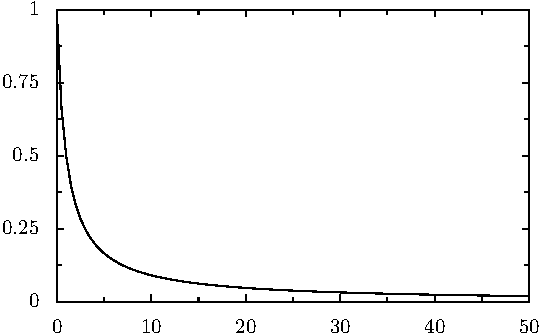
\includegraphics{function}')
\end{pycode}
\caption{$\frac{Vo(s)}{Vi(s)}=$$\frac{1}{1+s}$}
\end{figure}

Como a saída do circuito é obtida pelo capacitor, o circuito se configura como um filtro passa-baixas padrão. Para frequência igual a zero, o ganho em tensão é 1, e para frequencia no infinito o ganho em tensão é 0.
 

\section{Referências}


\bibliographystyle{sbc}
\bibliography{sbc-template}

\end{document}
